Una vez obtenidos y analizados los resultados de ambos experimentos, se realizará una comparación entre ambos. Como se ha mencionado anteriormente, la principal diferencia entre estos es la forma de dividir el conjunto de datos en los subconjuntos de entrenamiento y prueba.

El primer experimento tiene como ventaja principal la partición estratificada con \texttt{stratify} para mantener la proporción entre clases en ambos subconjuntos, la cual es especialmente útil en un conjunto de datos desbalanceado como el que se ha utilizado. Esto evita que las clases minoritarias tengan menor representación en el subconjunto de prueba o que directamente no aparezcan en este. Su principal desventaja es que con el conjunto de datos final generado en este trabajo, si existen muestras con el mismo \texttt{Flow ID} en ambos subconjuntos se introduce el problema de \texttt{data leakage}, donde el modelo encontraría patrones ya reconocidos durante el entrenamiento y produciría un falso aumento en las métricas de evaluación de este.

El segundo experimento tiene como ventaja principal que corrige el problema del primer experimento, evitando que muestras equivalentes aparezcan en ambos subconjuntos. Para lograrlo se dividen los subconjuntos por \texttt{Flow ID}, evitando que las muestras cuyo \texttt{Flow ID} sea el mismo (las cuales tendrán el mismo valor de las características definidas en el trabajo) aparezcan en ambos subconjuntos simultáneamente. Esto hace que la evaluación sea más estricta y se pueda evaluar de una forma más realista el rendimiento del modelo. La principal desventaja de este es que, aunque se evite el \texttt{data leakage}, no se puede garantizar que ambos subconjuntos estén balanceados, introduciendo la posibilidad de que haya clases infrarrepresentadas en el subconjunto de prueba o que directamente desaparezcan como es el caso de \texttt{Infiltration}.

Al comparar las matrices de confusión de ambos experimentos, se puede ver que para las clases mayoritarias se obtiene en ambas una gran tasa de aciertos en la diagonal principal. Esto es evidente en  las clases \texttt{BENIGN}, \texttt{DDoS}, \texttt{DoS GoldenEye}, \texttt{DoS Hulk}, \texttt{DoS slowloris}, \texttt{FTP-Patator}, \texttt{PortScan} y \texttt{SSH-Patator}, donde se obtienen valores de $1,00$ en ambos experimentos. 
En el caso de \texttt{DoS Slowhttptest}, en ambos experimentos se obtienen tasas de aciertos de $0,99$, con una ligera confusión de más en el experimento 2. Viendo los resultados de la clase \texttt{Bot}, se puede ver que en el experimento 2 se obtiene un $2\%$ más de aciertos. Esto puede deberse a que las muestras de esta clase en el subconjunto de pruebas en el segundo experimento sean más fáciles de clasificar que las del primero.
Los ataques web presentan la misma problemática en ambos experimentos, esta es, la confusión entre \texttt{Web Attack Brute Force} y \texttt{Web Attack XSS} y la confusión de \texttt{Web Attack Sql Injection} con tráfico benigno. En el caso de \texttt{Web Attack Brute Force}, los resultados son prácticamente idénticos, ambas tienen una tasa de acierto de $0,77$ y el resto se confunde con \texttt{Web Attack XSS}, habiendo un poco más de confusión en el experimento 2. Para \texttt{Web Attack Sql Injection}, el rendimiento es bajo en ambos experimentos. En el primer experimento se clasifican correctamente el $40\%$ de las muestras, mientras que en el segundo solo un $30\%$. En ambos la mayoría de confusiones son con tráfico benigno. En cuanto a \texttt{Web Attack XSS}, en ambos se muestran resultados muy similares, clasificándose en el primer experimento correctamente un $48\%$ de las muestras y en el segundo un $47\%$. La mayoría de errores vienen por la confusión con \texttt{Web Attack Brute Force}.
Las dos grandes diferencias son consecuencia de las estrategias de división. El primer caso es la clase \texttt{Infiltration}, la cual desaparece completamente de los resultados del experimento 2 debido a que, como se vio anteriormente, ninguna muestra es asignada al subconjunto de prueba. El segundo caso es la clase \texttt{Heartbleed}, en la cual en el experimento 1 se obtiene un resultado perfecto y en el 2 ningún acierto. Esto se puede deber a que en el experimento 1, las muestras de ambos subconjuntos sean las mismas y, por tanto, se reconozca un patrón y se clasifiquen correctamente. Esto es muy factible debido a que esta es una clase minoritaria y las muestras podrían compartir \texttt{Flow ID}. En el segundo experimento, al no reconocerse este patrón, el modelo falla en todos los casos.

En cuanto a la precisión global, esta varía muy poco entre ambos experimentos. Más concretamente, del primer al segundo experimento baja un $0,0018\%$. Esta bajada es leve porque la precisión global depende de las clases mayoritarias y en ambos experimentos se obtiene un rendimiento muy alto en estas.

Para ver con más detalle la diferencia entre ambos, se realiza una comparación entre los reportes de clasificación entre ambos experimentos. Esta se puede ver al completo en la tabla \ref{TAB:COMPARACION_REPORTS}. En esta, $P_n$ representa la precisión del experimento $n$, $R_n$ la exhaustividad, $F1_n$ la medida F1 y $S_n$ el soporte. Además, las columnas $\Delta P$, $\Delta R$, $\Delta F1$ y $\Delta S$ indican la variación entre el segundo y el primer experimento con respecto al experimento 2.

Como se puede observar, en más de la mitad de las clases los resultados son iguales obviando el soporte, el cual hace referencia al número de muestras de esa clase en el subconjunto de prueba. Esta diferencia se debe a que en el experimento 1 el número de muestras en este es del $25\%$ mientras que en el experimento 2 esto no se controla. Estas clases son \texttt{BENIGN}, \texttt{DDoS}, \texttt{DoS GoldenEye}, \texttt{DoS Hulk}, \texttt{FTP-Patator}, \texttt{PortScan}, \texttt{SSH-Patator} y \texttt{Web Attack Brute Force}. Con respecto a \texttt{Bot}, se observa un rendimiento ligeramente superior en el experimento 1. Si bien en el experimento 2 se clasifican correctamente un $2\%$ más de muestras dentro de la clase, un $4\%$ de las muestras pertenecen realmente a otra clase, haciendo que la medida F1 en este sea un $2\%$ menor. En cuanto a \texttt{DoS Slowhttptest}, se obtienen las mismas métricas pero se muestra que la medida F1 en el experimento 2 desciende un $1\%$, lo que indica que hay un rendimiento inferior pero prácticamente despreciable. Lo mismo sucede con \texttt{DoS slowloris}, donde en el experimento 2 la precisión desciende un $1\%$ pero la medida F1 es la misma debido a que esta bajada en la precisión será causada por un número muy bajo de muestras. Para \texttt{Web Attack XSS} se obtienen valores muy similares, en el experimento 1 la precisión y la exhaustividad son ligeramente superiores y eso causa que la medida F1 en el experimento 2 sea un $1\%$ menor. En el caso de \texttt{Web Attack Sql Injection} se observa una bajada más notable en el experimento 2. Aunque la precisión se mantiene en $1,00$ en ambos casos, la exhaustividad es un $10\%$ menor en el experimento 2, es decir, el modelo detecta una menor cantidad de muestras reales de esta clase, causando que la medida F1 sea un $11\%$ menor. La diferencia más evidente es en \texttt{Heartbleed}, donde en el experimento 1 se clasifican correctamente todas las muestras mientras que en el experimento 2 no se clasifica correctamente ninguna, probablemente debido a la explicación que se ha dado anteriormente. Finalmente, no se puede comparar \texttt{Infiltration} debido a que no hay ninguna muestra en el subconjunto de prueba del experimento 2.

\begin{table}{TAB:COMPARACION_REPORTS}{Comparación de los reportes de clasificación de ambos experimentos}
\centering
\scriptsize
\resizebox{\textwidth}{!}{
\begin{tabular}{p{4.2cm}ccc ccc ccc ccc}
\hline
Clase 
& P1 & P2 & \textbf{$\Delta$P}
& R1 & R2 & \textbf{$\Delta$R}
& F1-1 & F1-2 & \textbf{$\Delta$F1}
& S1 & S2 & \textbf{$\Delta$S} \\
\hline
BENIGN & 1.00 & 1.00 & \textbf{0.00} & 1.00 & 1.00 & \textbf{0.00} & 1.00 & 1.00 & \textbf{0.00} & 566672 & 571052 & \textbf{+4380} \\
Bot & 0.85 & 0.81 & \textbf{-0.04} & 0.95 & 0.97 & \textbf{+0.02} & 0.90 & 0.88 & \textbf{-0.02} & 491 & 467 & \textbf{-24} \\
DDoS & 1.00 & 1.00 & \textbf{0.00} & 1.00 & 1.00 & \textbf{0.00} & 1.00 & 1.00 & \textbf{0.00} & 32007 & 31983 & \textbf{-24} \\
DoS GoldenEye & 1.00 & 1.00 & \textbf{0.00} & 1.00 & 1.00 & \textbf{0.00} & 1.00 & 1.00 & \textbf{0.00} & 2573 & 2662 & \textbf{+89} \\
DoS Hulk & 1.00 & 1.00 & \textbf{0.00} & 1.00 & 1.00 & \textbf{0.00} & 1.00 & 1.00 & \textbf{0.00} & 57768 & 58118 & \textbf{+350} \\
DoS Slowhttptest & 1.00 & 1.00 & \textbf{0.00} & 0.99 & 0.99 & \textbf{0.00} & 1.00 & 0.99 & \textbf{-0.01} & 1375 & 1401 & \textbf{+26} \\
DoS slowloris & 1.00 & 0.99 & \textbf{-0.01} & 1.00 & 1.00 & \textbf{0.00} & 1.00 & 1.00 & \textbf{0.00} & 1449 & 1411 & \textbf{-38} \\
FTP-Patator & 1.00 & 1.00 & \textbf{0.00} & 1.00 & 1.00 & \textbf{0.00} & 1.00 & 1.00 & \textbf{0.00} & 1985 & 1996 & \textbf{+11} \\
Heartbleed & 1.00 & 0.00 & \textbf{-1.00} & 1.00 & 0.00 & \textbf{-1.00} & 1.00 & 0.00 & \textbf{-1.00} & 3 & 11 & \textbf{+8} \\
Infiltration & 1.00 & -- & \textbf{--} & 0.67 & -- & \textbf{--} & 0.80 & -- & \textbf{--} & 9 & 0 & \textbf{-9} \\
PortScan & 0.99 & 0.99 & \textbf{0.00} & 1.00 & 1.00 & \textbf{0.00} & 1.00 & 1.00 & \textbf{0.00} & 39731 & 39748 & \textbf{+17} \\
SSH-Patator & 1.00 & 1.00 & \textbf{0.00} & 1.00 & 1.00 & \textbf{0.00} & 1.00 & 1.00 & \textbf{0.00} & 1474 & 1354 & \textbf{-120} \\
Web Attack Brute Force & 0.78 & 0.78 & \textbf{0.00} & 0.77 & 0.77 & \textbf{0.00} & 0.77 & 0.77 & \textbf{0.00} & 377 & 375 & \textbf{-2} \\
Web Attack Sql Injection & 1.00 & 1.00 & \textbf{0.00} & 0.40 & 0.30 & \textbf{-0.10} & 0.57 & 0.46 & \textbf{-0.11} & 5 & 10 & \textbf{+5} \\
Web Attack XSS & 0.49 & 0.48 & \textbf{-0.01} & 0.48 & 0.47 & \textbf{-0.01} & 0.48 & 0.47 & \textbf{-0.01} & 163 & 157 & \textbf{-6} \\
\hline
Macro avg & 0.94 & 0.86 & \textbf{-0.08} & 0.88 & 0.82 & \textbf{-0.06} & 0.90 & 0.83 & \textbf{-0.07} & 706082 & 710745 & \textbf{+4663} \\
Weighted avg & 1.00 & 1.00 & \textbf{0.00} & 1.00 & 1.00 & \textbf{0.00} & 1.00 & 1.00 & \textbf{0.00} & 706082 & 710745 & \textbf{+4663} \\
\hline
\end{tabular}
}
\end{table}

Finalmente, se compara la importancia de características de ambos experimentos. Como se puede ver, aunque los valores difieran, las 8 primeras características se mantienen en orden, siendo estas además las características definidas y añadidas en este trabajo para enriquecer el conjunto de datos. Dentro de la importancia de ambos experimentos, hay algunas características exclusivas de cada uno, pero como vienen de serie en el conjunto de datos se omiten, por lo que se van a comparar los valores de las comunes a ambos experimentos. Aunque los valores difieran un poco, lo importante es que la estrategia de partición no afecta a la relevancia de las nuevas características para clasificar las muestras. Se puede ver una representación visual de esta comparación en la figura \ref{FIG:COMPARACION_IMPORTANCE}.

\begin{figure}[htb]
    \centering
    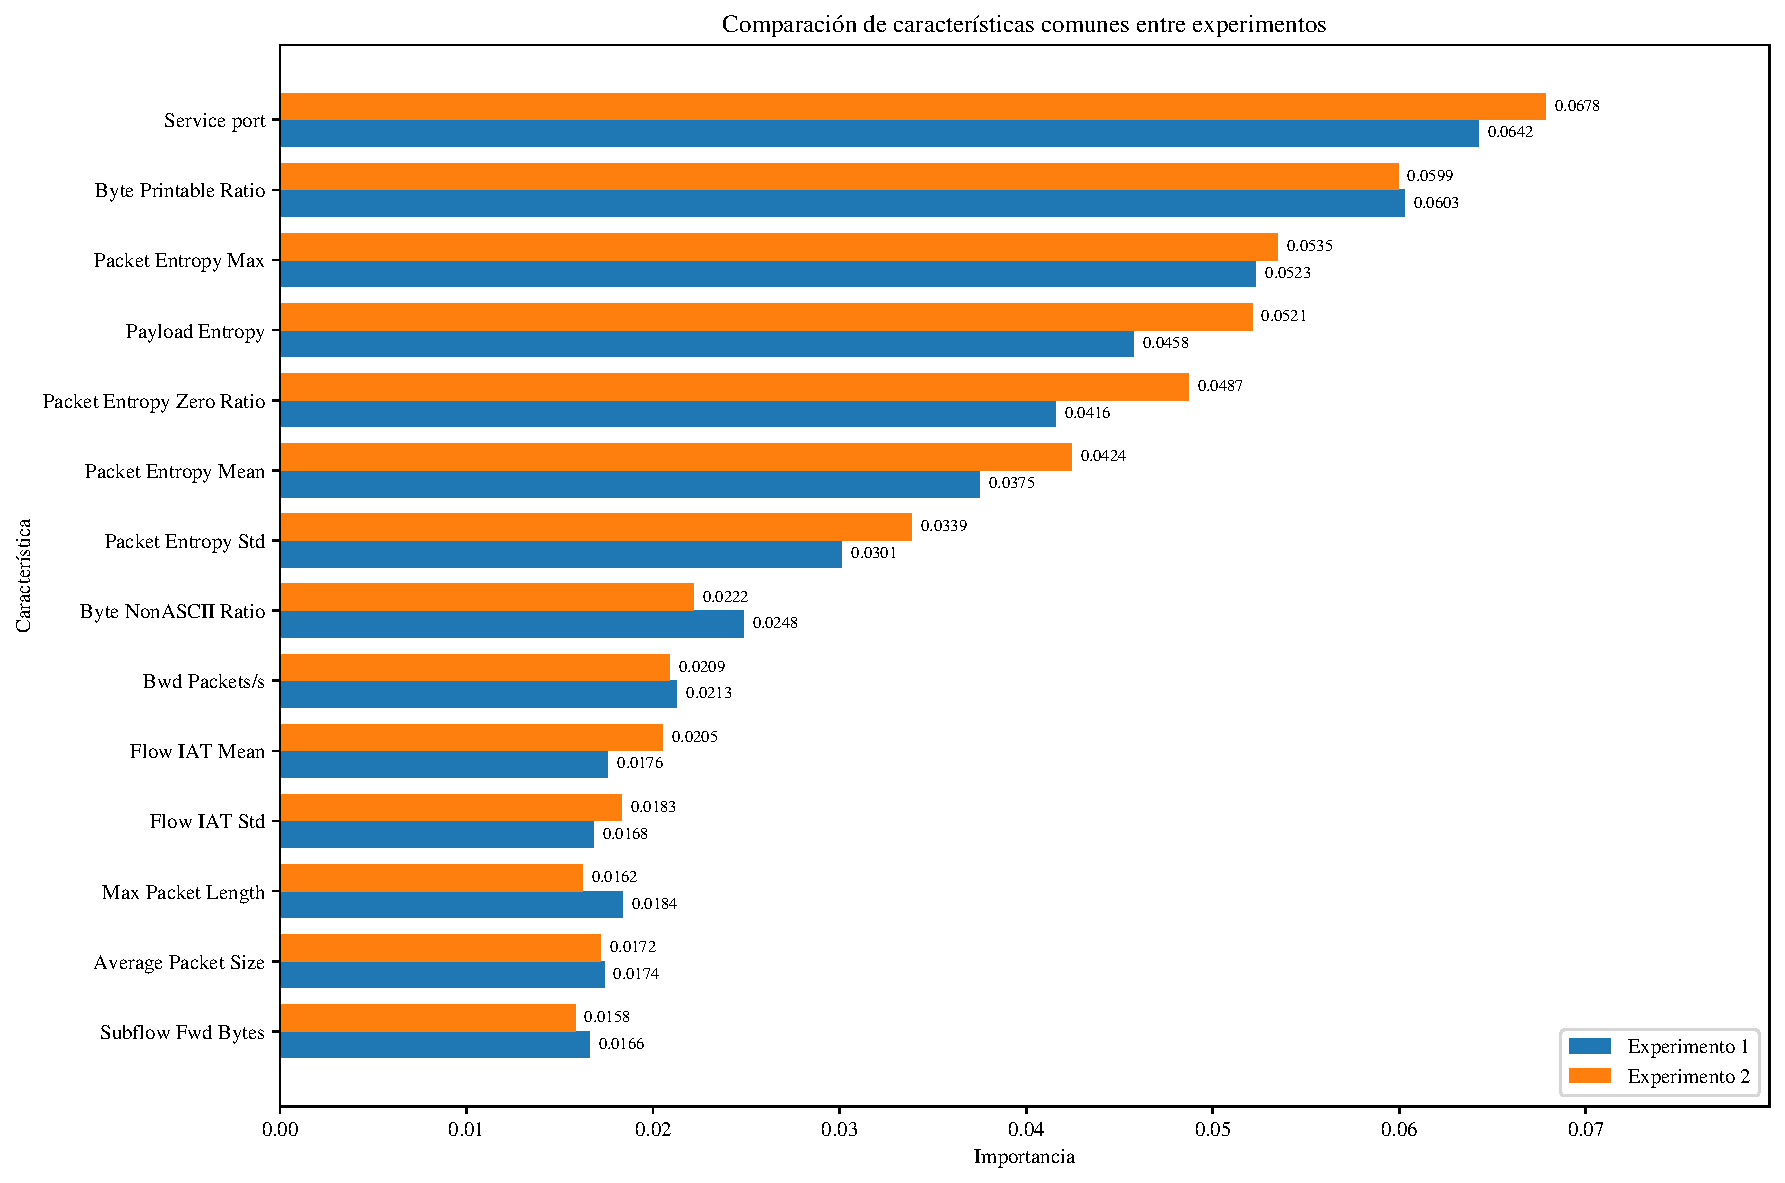
\includegraphics[width=.90\textwidth]{img/comparacion_feature_importance_comunes.pdf}
    \caption{Comparación de la importancia de características comunes a ambos experimentos}\label{FIG:COMPARACION_IMPORTANCE}
\end{figure}